\newcommand{\CLASSINPUToutersidemargin}{0.5in}
\documentclass[a4paper,conference]{IEEEtran}
\IEEEoverridecommandlockouts
% The preceding line is only needed to identify funding in the first footnote. If that is unneeded, please comment it out.
\usepackage{cite}
\usepackage{amsmath,amssymb,amsfonts}
\usepackage{algorithmic}
\usepackage{graphicx}
\usepackage{textcomp}
% \usepackage{xeCJK}
% \setCJKmainfont{Noto Sans Mono CJK TC}
\usepackage{xcolor}
\usepackage{xurl}
\usepackage{hyperref}
\hypersetup{
    colorlinks = true,
    linkcolor = [rgb]{.1,.1,.44},
    urlcolor = blue,
    citecolor = [rgb]{.0,.39,.0}
}
\usepackage{listings}
\usepackage{color}
\definecolor{dkgreen}{rgb}{0,0.6,0}
\definecolor{gray}{rgb}{0.5,0.5,0.5}
\definecolor{mauve}{rgb}{0.58,0,0.82}
\lstset{frame=tb,
  language=Java,
  aboveskip=3mm,
  belowskip=3mm,
  showstringspaces=false,
  columns=flexible,
  basicstyle={\small\ttfamily},
  numbers=none,
  numberstyle=\tiny\color{gray},
  keywordstyle=\color{blue},
  commentstyle=\color{dkgreen},
  stringstyle=\color{mauve},
  breaklines=true,
  breakatwhitespace=true,
  tabsize=3
}
\def\BibTeX{{\rm B\kern-.05em{\sc i\kern-.025em b}\kern-.08em
    T\kern-.1667em\lower.7ex\hbox{E}\kern-.125emX}}
\begin{document}

\renewcommand\footnoterule{{\hrule height 0.5pt}\vspace{0.04in}}
\def\IEEEkeywordsname{Keywords}

\title{Context-based Arithmetic Coding Homework\\
\vspace{-0.1in}
{\normalsize Authors Name, Student ID}
}

\author{}

\maketitle

\vspace{0.1in}

\begin{IEEEkeywords}
Arithmetic Coding, Context-based, Prediction with Partial Matching, Data Compression
\end{IEEEkeywords}

\section{Introduction}

In this homework, I implement the context-based arithmetic coding algorithm, and compare the performance of fixed probability model and context-based arithmetic coding algorithm.

\section{Arithmetic Coding Algorithm}

Arithmetic coding is a coding technique that maps a string of symbols to a real number in the interval $[0, 1)$. In arithmetic coding, coders maintain a current interval $[l, u)$, and the next symbol is encoded by narrowing the interval to a subinterval of $[l, u)$. The subinterval is determined by the probability of the next symbol. The decoder can reconstruct the original string by decoding the real number back to the string of symbols.

There is an integer implementation of arithmetic coding, that use a $b$-bit integer $x$ to represent a fixed-point number $x / 2^b$ in the interval $[0, 1)$, and the coder maintains a current interval $[l, u)$ as a pair of $b$-bit integers, and keep scaling the interval to prevent integer underflow.

\section{Fixed Probability Model}

In fixed probability model, the encoder estimates the probability distribution of the symbols from the input string, and the decoder uses the same probability distribution to decode the symbols. The compressed file format must include the probability distribution of the symbols.

\subsection{Compressed File Format}

For simplicity, I put the size of input file in the header of the compressed file, instead of the end of sequence (EOS) symbol. The compressed file format is as follows:

\begin{itemize}
    \item Header: size of input file
    \item Header: probability distribution of the symbols
    \item Data: compressed data
\end{itemize}

\section{Context-based Arithmetic Coding Algorithm - Prediction with Partial Matching}

In context-based arithmetic coding, the encoder and decoder use the same context model to estimate the probability distribution of the symbols, and the context model can be update after each symbol is encoded or decoded. One of the context model is prediction with partial matching (PPM).

\subsection{Order of Context}

In PPM model, there is a parameter $n$ that is the order of the context. The $k$ order context is a string of $k$ symbols, and the probability distribution of the next symbol is estimated from the context. The context is updated after each symbol is encoded or decoded.

\subsection{Escape Symbol}

There is a special symbol, escape symbol, that is used when the symbol is not found in the context. There are several ways to design the probability distribution of the escape symbol, in this homework, I follow PPMA method, which is to set the probability of the escape symbol to one in the context.

When the symbol is not found in the context, the encoder encodes the escape symbol and go to the next order context. When the symbol is not found in the order 0 context, the encoder encodes the escape symbol and output the symbol directly.

\subsection{Exclusion Principle}

There is a way to improve the performance of PPM, which is exclusion principle. The exclusion principle is to exclude the symbol that is has been present in the higher order context. For example, if the symbol is present in the order 2 context, then the probability of the symbol in the order 1 context is set to zero.

\section{Implementation}

\subsection{Arithmetic Coding}

The arithmetic coding is implemented in \texttt{Arithmetic} class. The \texttt{send} method is used to encode a symbol, and the \texttt{recv} method is used to decode a symbol, and the \texttt{update} method is used to update the interval after each symbol is encoded or decoded. The \texttt{end} method is used to flush the remaining bits in the interval.

The \texttt{end} function didn't mention in the textbook, but when I write the decoder, I found that the decoder cannot correctly decode the last symbol. I think the reason is that I didn't use EOS symbol, so I need to flush the remaining bits in the interval. After I add the \texttt{end} function, the decoder can correctly decode the last symbol for majority of the cases.

\subsection{Fixed Probability Model}

The fixed probability model is implemented in \texttt{ArithmeticFPM} class. The probability distribution of the symbols is estimated from the input string, and the probability distribution is stored in the header of the compressed file.

\subsection{Prediction with Partial Matching Model}

The PPM model is implemented in \texttt{ArithmeticPPM} and \texttt{Context} class, and the \texttt{Context} class is used to store the context model. The \texttt{ArithmeticPPM} class is used to send and receive symbols, and update the context model after each symbol is encoded or decoded.

I use a trie to store the $n$ order context model instead of a hash table, because the trie has a better performance than the hash table in time and space complexity. The trie is a tree structure, and from the root to the leaf is a string of symbols, and each node in the trie stores the count of the symbols.

\section{Experimental Results}

\subsection{Fixed Probability Model}

The compression ratio of fixed probability model is shown in Fig.~\ref{fig-chart-fpm-comp}.

The \texttt{basic-8} and \texttt{basic-32} are the basic huffman coding with 8-bit and 32-bit, and the \texttt{fpm.1} and \texttt{fpm.8} are the 1-bit and 8-bit fixed probability model, corresponding to 2 and 256 symbols.

I have compared the compression ratio of fixed probability model with other implementations, scuh as \texttt{libcoders} \cite{libcoders} and \texttt{ref-Arithmetic} \cite{Reference-arithmetic-coding}, we can see that the compression ratio of fixed probability model are similar to other implementations.
One thing to note is that the \texttt{libcoders} failed to decode the last symbol for \texttt{alexnet.pth}.

The figure shows that the 1-bit fixed probability model have rough same size as original file, and the 8-bit fixed probability model has a little better compression ratio than 8-bit huffman coding, but much worse than 32-bit huffman coding.

\begin{figure}[htbp]
\centerline{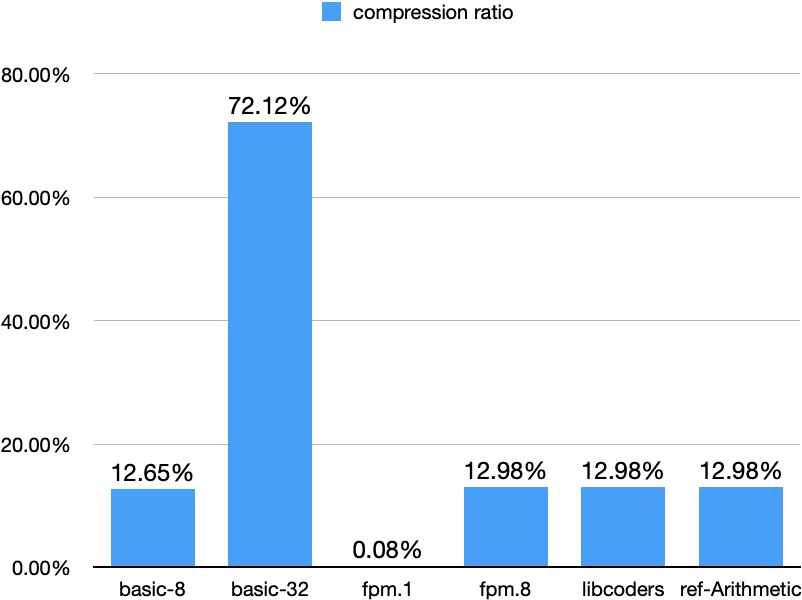
\includegraphics[height=6.15cm, keepaspectratio,]{assets/chart-fpm-comp.png}}
\caption{The compression ratio of fixed probability model compare to huffman coding}
\label{fig-chart-fpm-comp}
\end{figure}

\subsection{Prediction with Partial Matching Model}

The compression ratio of PPM model with different order is shown in Fig.~\ref{fig-chart-ppm-1} and Fig.~\ref{fig-chart-ppm-8}. The \texttt{ppm.1.-1} means the 1-bit PPM model with -1 order context, which means the context is not used. The \texttt{ppm.8.3} means the 8-bit PPM model with 3 order context.

From the figure, we can see that -1 order context didn't improve the compression ratio, and the 1-bit PPM model with 0 order context has similar compression ratio as 1-bit fixed probability model, and when the order of the context is increased, the compression ratio is increased.

Worth to note that the 1-bit PPM model with 3 order context has highest compression ratio for 1-bit PPM model for \texttt{alexnet.pth}, but the last symbol cannot be decoded correctly.

\begin{figure}[htbp]
\centerline{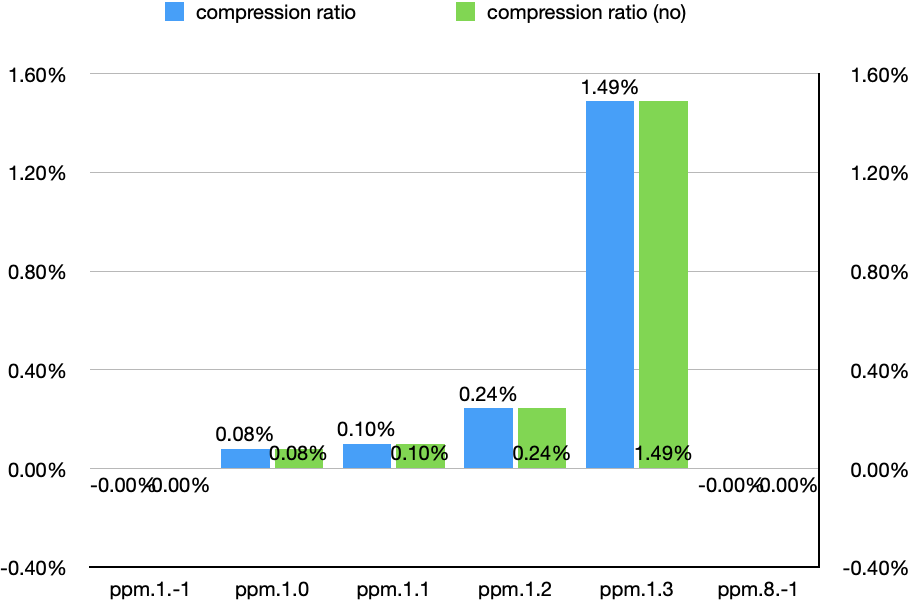
\includegraphics[height=6.15cm, keepaspectratio,]{assets/chart-ppm-1-2.png}}
\caption{The compression ratio of 1-bit PPM model with different order}
\label{fig-chart-ppm-1}
\end{figure}

Compare two figure, 8-bit PPM model has much better compression ratio than 1-bit PPM model, and the compression ratio of 8-bit PPM model with 0 context is similar to 8-bit huffman coding, and 3 order context has close compression ratio as 32-bit huffman coding.

According to the figure, we can known that the exclusion principle can improve the compression ratio, but the improvement is not obvious. I think the reason is that the exclusion principle only exclude the symbol that is present in the higher order context, but the order I used is not high enough, so the improvement is not obvious.

\begin{figure}[htbp]
\centerline{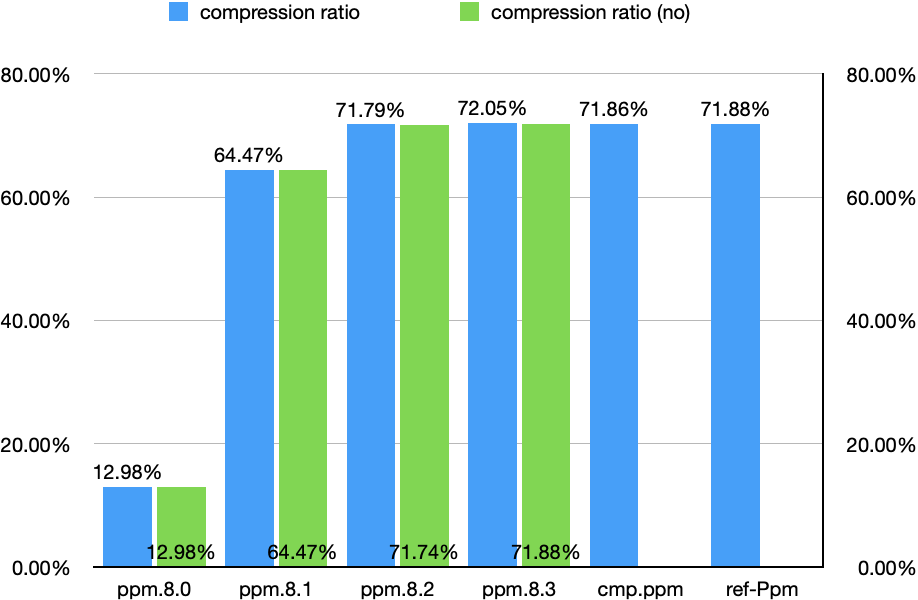
\includegraphics[height=6.15cm, keepaspectratio,]{assets/chart-ppm-8-cmp-2.png}}
\caption{The compression ratio of 8-bit PPM model with different order}
\label{fig-chart-ppm-8}
\end{figure}


\begin{figure*}[htbp]
\centerline{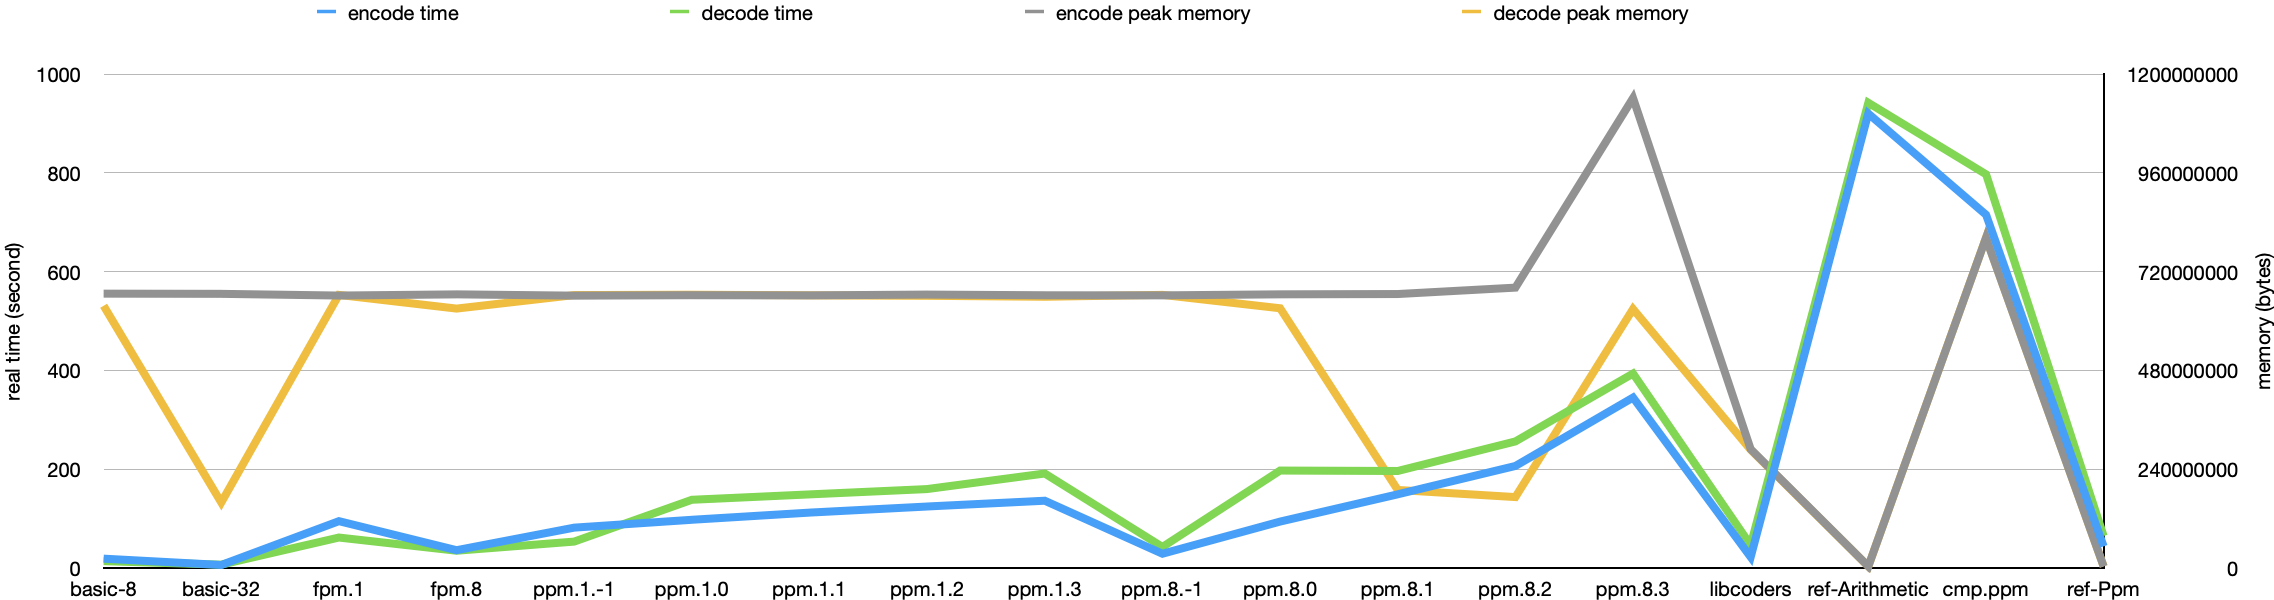
\includegraphics[width=20cm, keepaspectratio,]{assets/chart-perf.png}}
\caption{The time and memory usage of different algorithms and parameters.}
\label{fig-chart-perf}
\end{figure*}

The \texttt{ref-Ppm} are the PPM implementation from Reference-arithmetic-coding\cite{Reference-arithmetic-coding}, and the \texttt{cmp.ppm} is the implementation from rene-puschinger/ppm\cite{rene-puschinger/ppm}.
From the figure, we can see that my implementation of PPM model has similar compression ratio as other implementations.


\subsection{Performance}

The performance of fixed probability model and PPM model is shown in Fig.~\ref{fig-chart-perf}.
The \texttt{ref-Arithmetic} and \texttt{ref-Ppm} are the implementation from Reference-arithmetic-coding\cite{Reference-arithmetic-coding}, and the \texttt{libcoders} is the implementation from libcoders\cite{libcoders}, and the \texttt{cmp.ppm} is the implementation from rene-puschinger/ppm\cite{rene-puschinger/ppm}.

From the chart, we can see that my implementation of fpm and ppm has similar memory usage, and as the ppm order increase, the memory and time usage is increased.

For fixed probability model, the \texttt{libcoders} has the best time performance, and the \texttt{ref-Arithmetic} has the best memory performance.

For PPM model, the \texttt{ref-Ppm} has the best time and memory performance.
Worth to note that the \texttt{cmp.ppm} has the worst time performance, because it use 5 order context, but compression ratio is not better than 3 order context in my implementation.
In my implementation, the encoding time is a little shorter than decoding time, and the memory usage of encoding is a little higher than decoding.

\section{Conclusion}

In this homework, I have implemented the fixed probability model and PPM model, and compared the compression ratio and performance with other implementations.
The result shows that 8-bit PPM model with 3 order context has close compression ratio as 32-bit huffman coding, and the exclusion principle can improve the compression ratio, but the improvement is not obvious.

There are some problems in my implementation, such as the last symbol cannot be decoded correctly for some case in PPM model, and the performance is not good enough, so I can't run the experiment with higher order context.

\section{Appendix}

\subsection{Experiment Environment}

\begin{itemize}
\item CPU: Apple M1 Pro 8-Core (6 Performance / 2 Efficiency)
\item Memory: 16GB
\item Compiler: Apple clang version 14.0.3 \\ (clang-1403.0.22.14.1)
\item Measurement: /usr/bin/time -l -h -p
\end{itemize}

\subsection{Usage}

\begin{lstlisting}[escapeinside={(*}{*)}]
Usage: ./bin/release/arithmetic-coding.exe -t <type> [-e | -d] [options...] [-b <bits>] [-i <file>] [-o <file>]
    -t, --type <type>       Set coding algorithm
    -e, --encode            Encode
    -d, --decode            Decode
    -i, --input <file>      Set input file (default STDIN)
    -o, --output <file>     Set output file (default STDOUT)
    -b, --bits <bits>       Tread input file as <bits> data source (default 8) (1 / 8)
    -n, --order <order>     Set PPM context order (default 2)
    -v, --verbose           Show debug / analysis /time info
    --pmf                   Show pmf freq
    --no-time               No show time info
    --no-skip               No excludesive in ppm
    -h, --help              Show this help

Coding Algorithms
    arithmetic-ppm  Context Arithmetic Coding Algorithm (Prediction with Partial Match)
    arithmetic-fpm  Arithmetic Coding Algorithm (Fixed Probability Model)
\end{lstlisting}

\begin{thebibliography}{00}
\bibitem{Introduction to Data Compression} Sayood, K. (2014), Introduction to Data Compression (4th Edition). Morgan Kaufmann
\bibitem{libcoders} \url{https://github.com/snovvcrash/libcoders}
\bibitem{rene-puschinger/ppm} \url{https://github.com/rene-puschinger/ppm}
\bibitem{Reference-arithmetic-coding} \url{https://github.com/nayuki/Reference-arithmetic-coding}
\end{thebibliography}

\end{document}
